\documentclass[colorlinks = true, allcolors = black, ngerman, 11pt,
a4paper, twoside, titlepage]{article}
\usepackage[utf8]{inputenc}
\usepackage[T1]{fontenc}
\usepackage{lmodern}
\usepackage{amsmath}

\usepackage{mathtools}
\usepackage{amssymb}
\usepackage{graphicx}
\usepackage[left=2.1cm, right=2.1cm, top=1.7cm,
bottom=1.7cm,includehead,includefoot]{geometry}
\usepackage[margin=1.9cm,format=hang]{caption}
\usepackage[ngerman]{babel}
\usepackage{nameref}

%use tables that fill textwidth
\usepackage{tabularx}
\usepackage{makecell}
%used for tables with merged rows
\usepackage{multirow}
%double horizontal line
\usepackage{hhline}
%better newlines
\usepackage{parskip}

%setting to allow the captions to count based on the section they are in

\numberwithin{figure}{section}

\usepackage{siunitx}
\usepackage{cancel}

\usepackage[colorlinks=true,allcolors=black]{hyperref}

%package to reference figures and tables as [environment].
% [Section].[Subsection]...
\usepackage{cleveref}

\usepackage{subfiles}

\usepackage{subcaption}

%einheiten
\renewcommand{\si}[2]{\SI{#1}{#2}}
\begin{document}
	
	\section{\huge Weihnachtsaufgabe: Permittivität bestimmen}
	
	In dieser Aufgabe ging es darum, die Permittivität von zwei
	unterschiedlichen Materialien zu bestimmen, mittels des Satz von Snellius.
	Das erste Material war Gelatine, welches vorgegeben war, beim zweiten
	Material handelt es sich um einen durchsichtigen Kunststoffwürfel.
	
	\subsection{Gelatine} \label{sec:gealtine}
	\paragraph{Aufbau}
	Für dieses Experiment wurden $\si{33}{\gram}$ Gelatine (siehe Marke
	in \cref{fig:gelatinebeutel}) auf $\si{64}{\gram}$ Wasser verwendet.
	Als Gussform wurde ein zylindrisches Trinkglas verwendet.
	Der Gelatine Block wurde anschließend mit einem Messer zugeschnitten,
	um möglichst viele Luftbläschen aus dem Block zu schneiden und
	möglichst glatte Flächen zu haben.
	
	\begin{figure}[h]
		\centering
		\begin{subfigure}{0.4\textwidth}
			\centering
			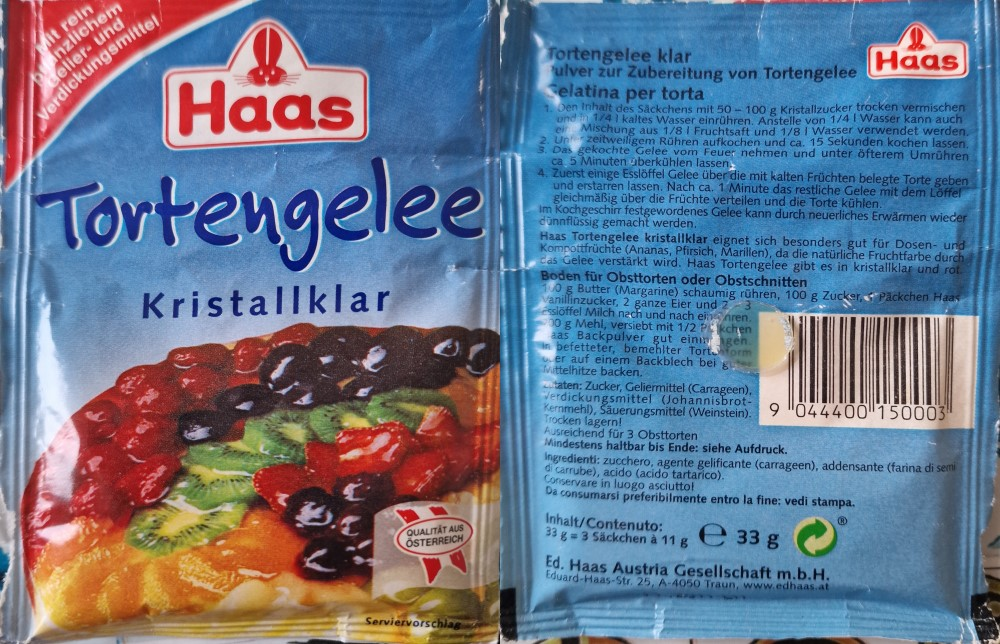
\includegraphics[height=0.7\textwidth]{imgs/gelatine_beutel}
			\caption{Marke der Gelatine}
			\label{fig:gelatinebeutel}
		\end{subfigure}
		\hfil
		\begin{subfigure}{0.4\textwidth}
			\centering
			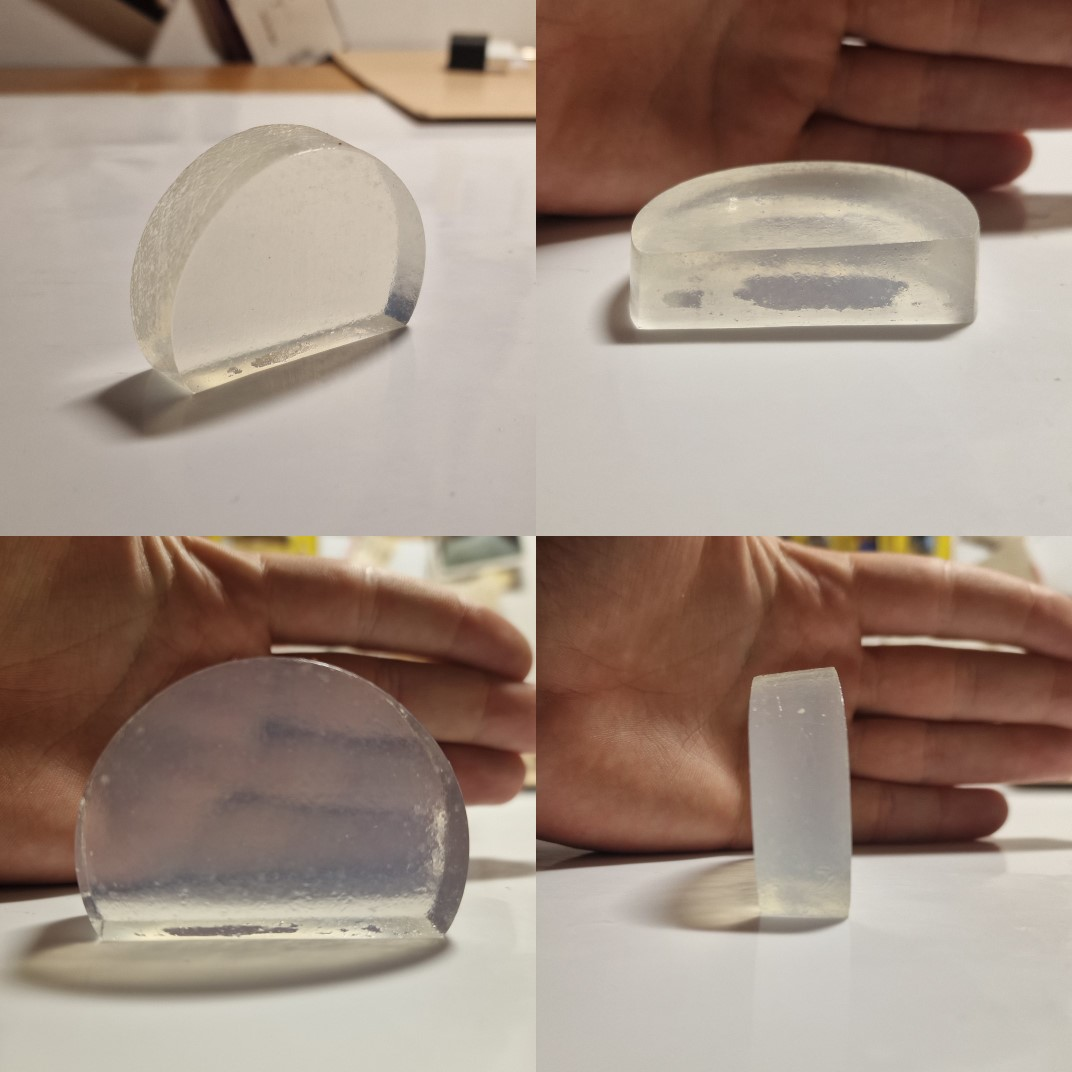
\includegraphics[height=0.7\textwidth]{imgs/gelatine_ansichten}
			\caption{Resultat Gelatine}
			\label{fig:gelatineansichten}
		\end{subfigure}
		\caption{Gelatine Sample}
		\label{figs:gelatine-beutel-sample}
	\end{figure}
	
	In \cref{figs:messaufbau-gelatine} ist der Messaufbau zu sehen. Es
	wurden 2 Geodreiecke mit Klebeband verklebt.
	\begin{figure}[h]
		\centering
		\begin{subfigure}{0.4\textwidth}
			\centering
			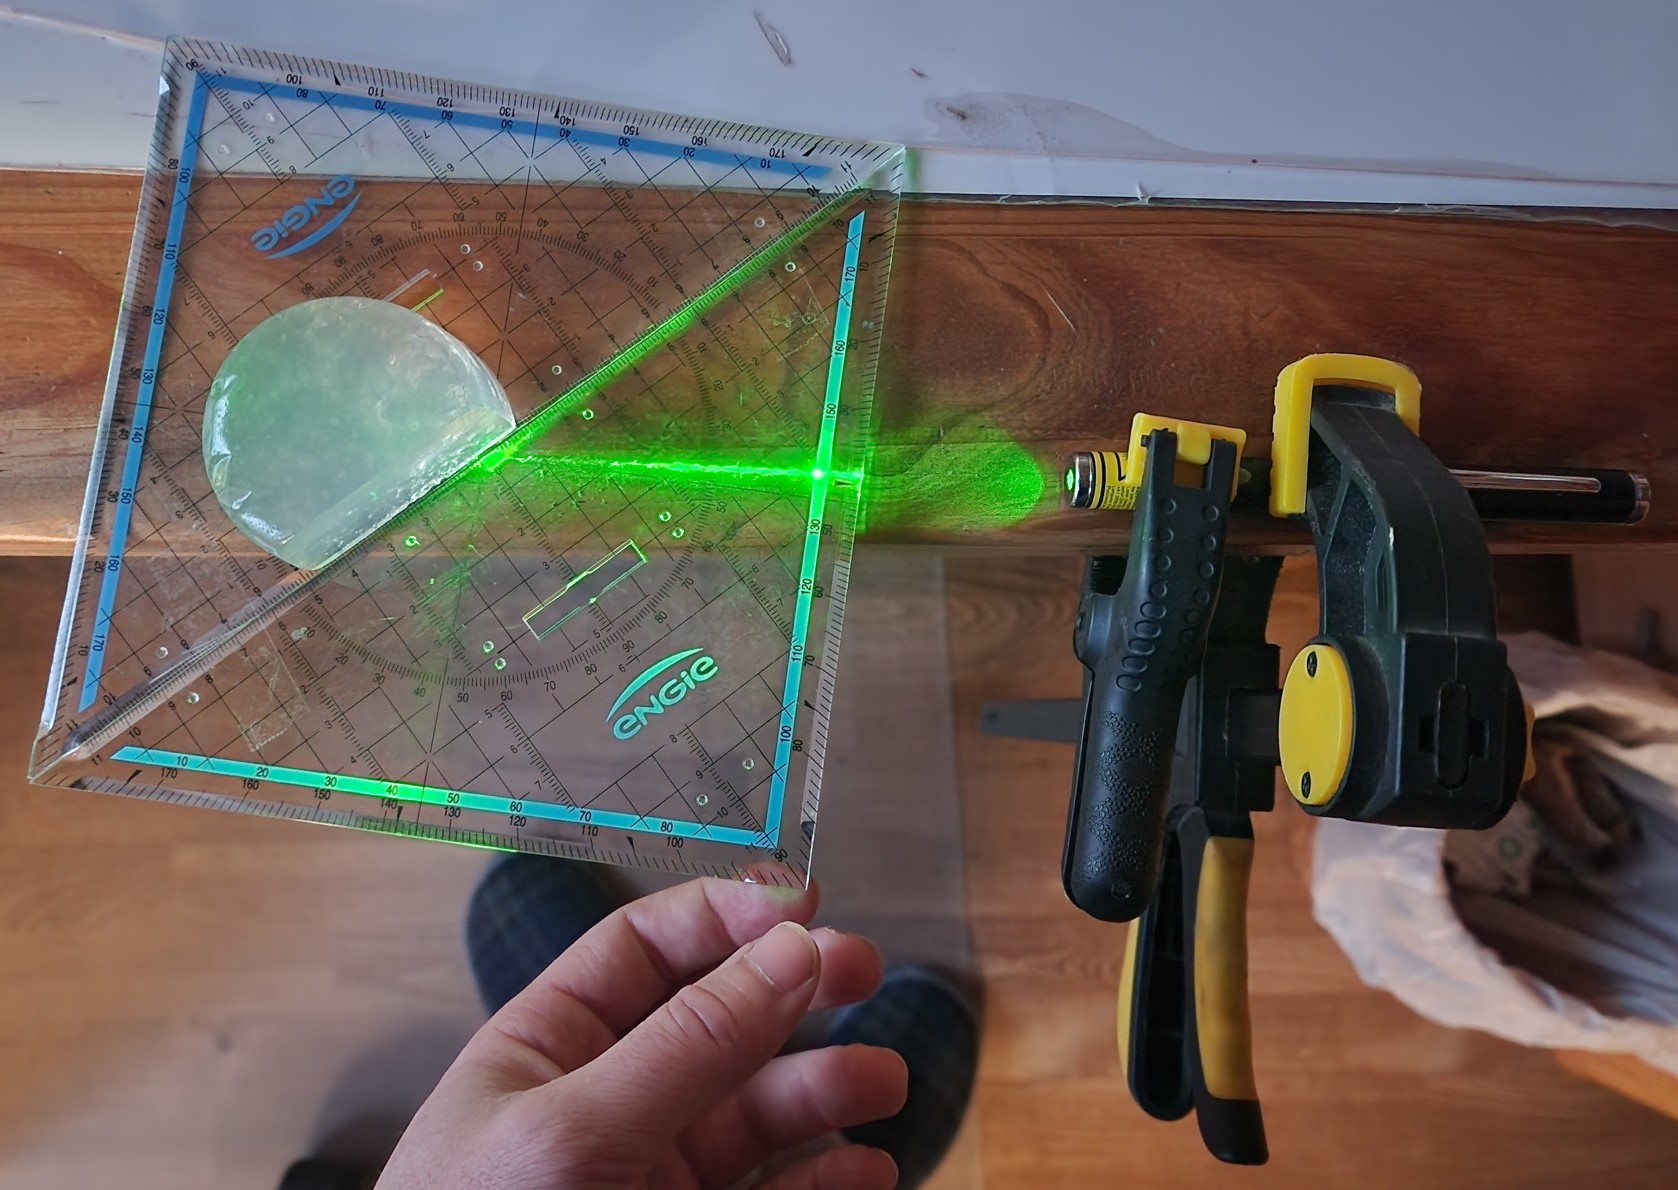
\includegraphics[height=0.7\linewidth]{imgs/winkel_einstellen_gelatine}
			\caption{Einfallswinkel einstellen}
			\label{fig:winkeleinstellengelatine}
		\end{subfigure}
		\hfil
		\begin{subfigure}{0.4\textwidth}
			\centering
			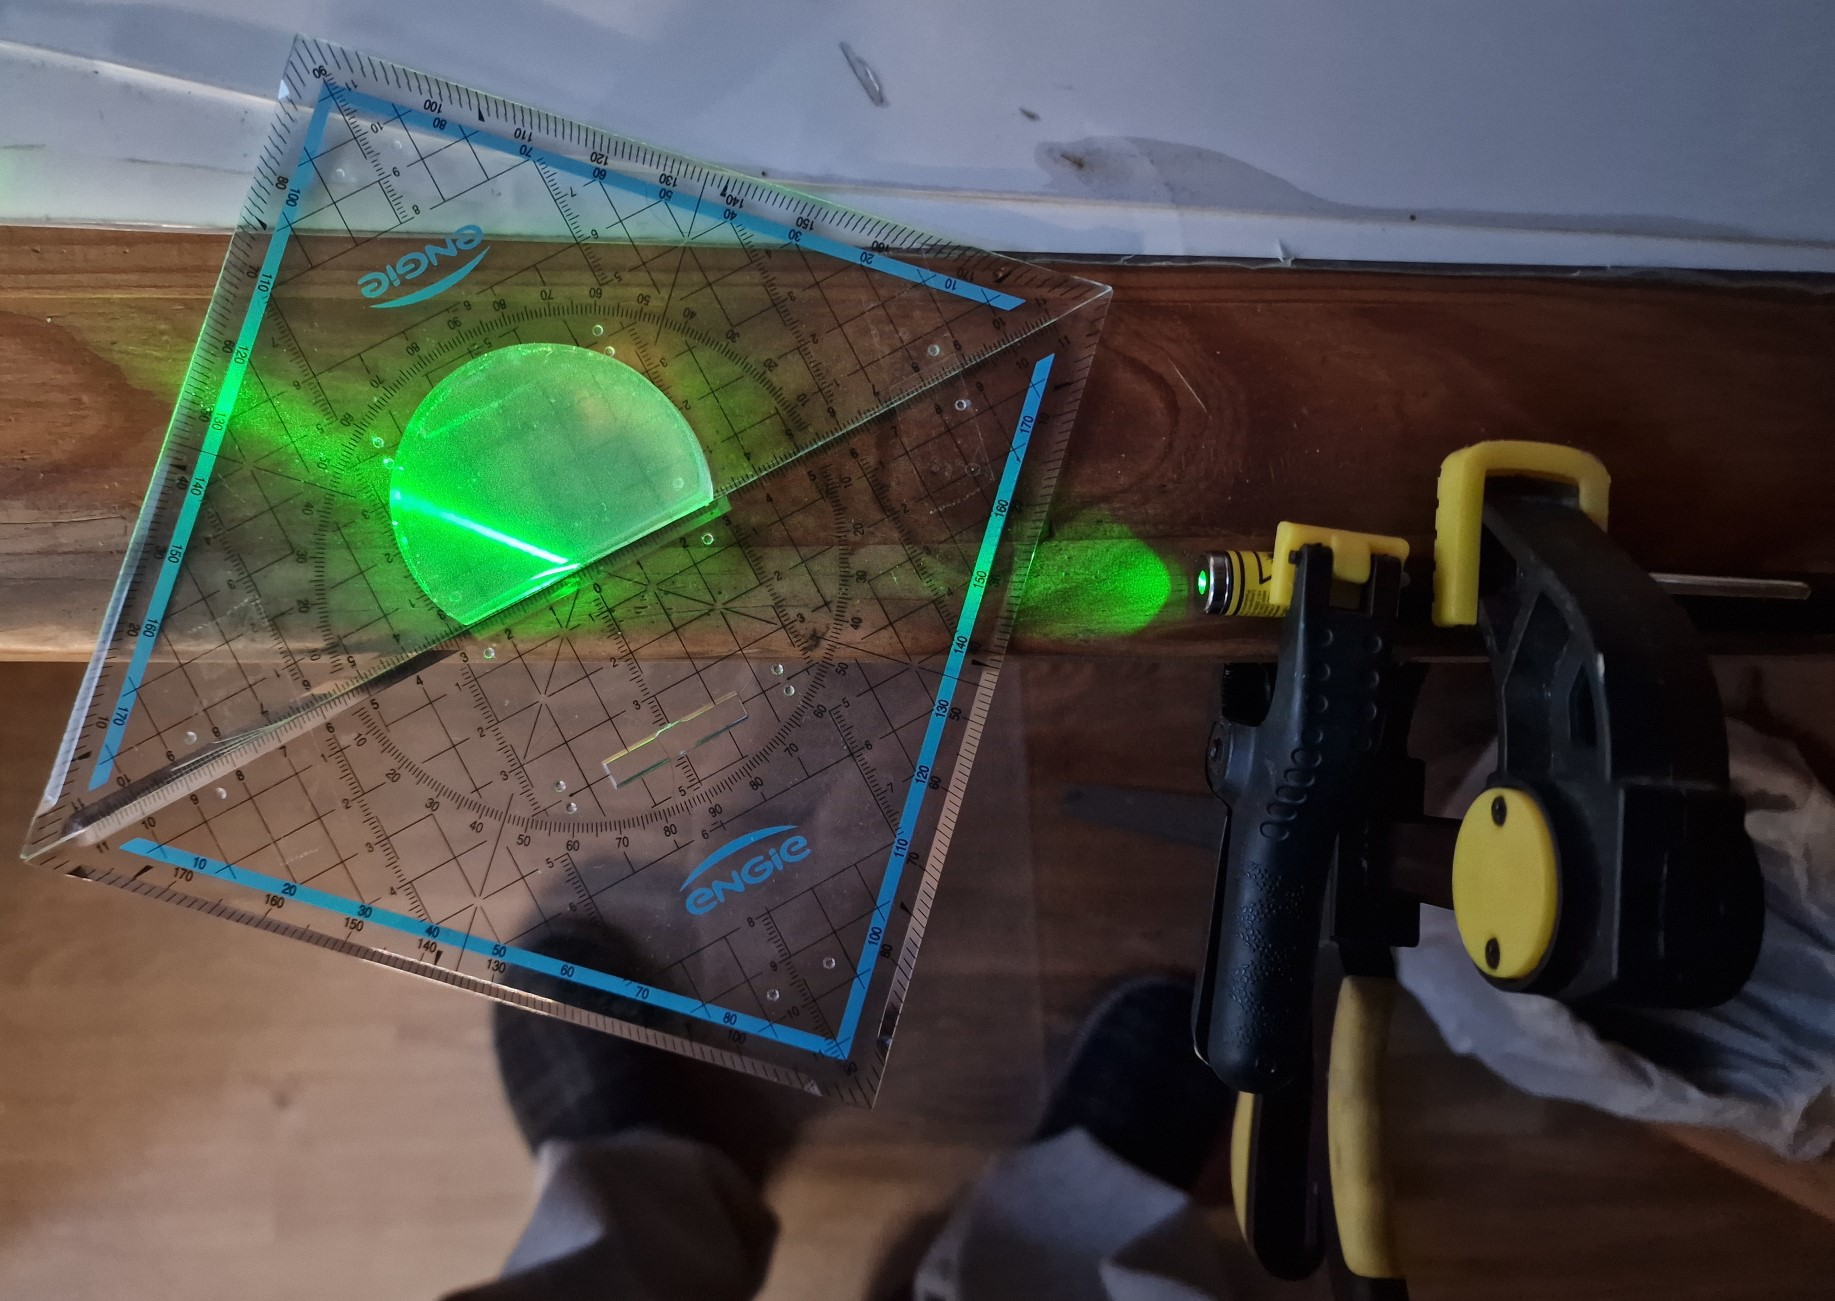
\includegraphics[height=0.7\linewidth]{imgs/winkel_messen_gelatine}
			\caption{Transmissionswinkel messen}
			\label{fig:winkelmessengelatine}
		\end{subfigure}
		\caption{Messaufbau mit Gelatine}
		\label{figs:messaufbau-gelatine}
	\end{figure}
	
	
	
	\paragraph{Messung}
	
	Alle Winkel sind vom Lot aus gemessen, das heißt von der
	\(\si{90}{\degree}\) Markierung des Geodreiecks.
	Mit \cref{eqn:eps_r} konnte die Relative Permittivität ermittelt werden.
	\begin{equation} \label{eqn:eps_r}
		\frac{\sin\Theta_{1}}{\sin\Theta_{2}} = \frac{n_{2}}{n_{1}} =
		\sqrt{\frac{\varepsilon_{2}}{\varepsilon_{1}}}=\sqrt{\varepsilon_{2}}
	\end{equation}
	
	
	
	In \cref{tab:gelatine-messergebnisse} sind die Messergebnisse zu sehen.
	\begin{table} [h]
		\centering
		\begin{tabular}{|c|c|c|c|c|c|}
			\hline
			Einfallswinkel $\Theta_{e}$ & $\si{15}{\degree}$ &
			$\si{30}{\degree}$ & $\si{45}{\degree}$ & $\si{60}{\degree}$ &
			$\si{80}{\degree}$ \\
			\hline
			Transmissionswinkel $\Theta_{t}$ & $\si{10}{\degree}$ &
			$\si{21}{\degree}$ & $\si{31}{\degree}$ & $\si{42}{\degree}$ &
			$\si{48}{\degree}$ \\
			\hline
			Brechungsindex $n$ & 1.490 & 1.395 & 1.373 & 1.294 & 1.325 \\
			\hline
			Relative Permittivität $\varepsilon_{r}$ & 2.220 & 1.946 & 1.885
			& 1.674 & 1.756 \\
			\hline
		\end{tabular}
		\caption{Mess- und Rechenergebnisse für die Gelatine}
		\label{tab:gelatine-messergebnisse}
	\end{table}
	
	Damit kommt man auf eine mittlere Relative Permittivität
	$\bar{\varepsilon}_{r} = 1.896$ und einen Brechungsindex $\bar{n} = 1.375$
	
	
	\subsection{Kunststoff Würfel}
	\paragraph{Aufbau}
	Als zweites Testobjekt wurde ein durchsichtiger Kunststoffwürfel
	genommen, dessen Material nicht bekannt ist. Er ist in zu sehen. Der
	Messaufbau ist gleich wie in \cref{sec:gealtine}.
	\begin{figure}[h]
		\centering
		\begin{subfigure}{0.4\textwidth}
			\centering
			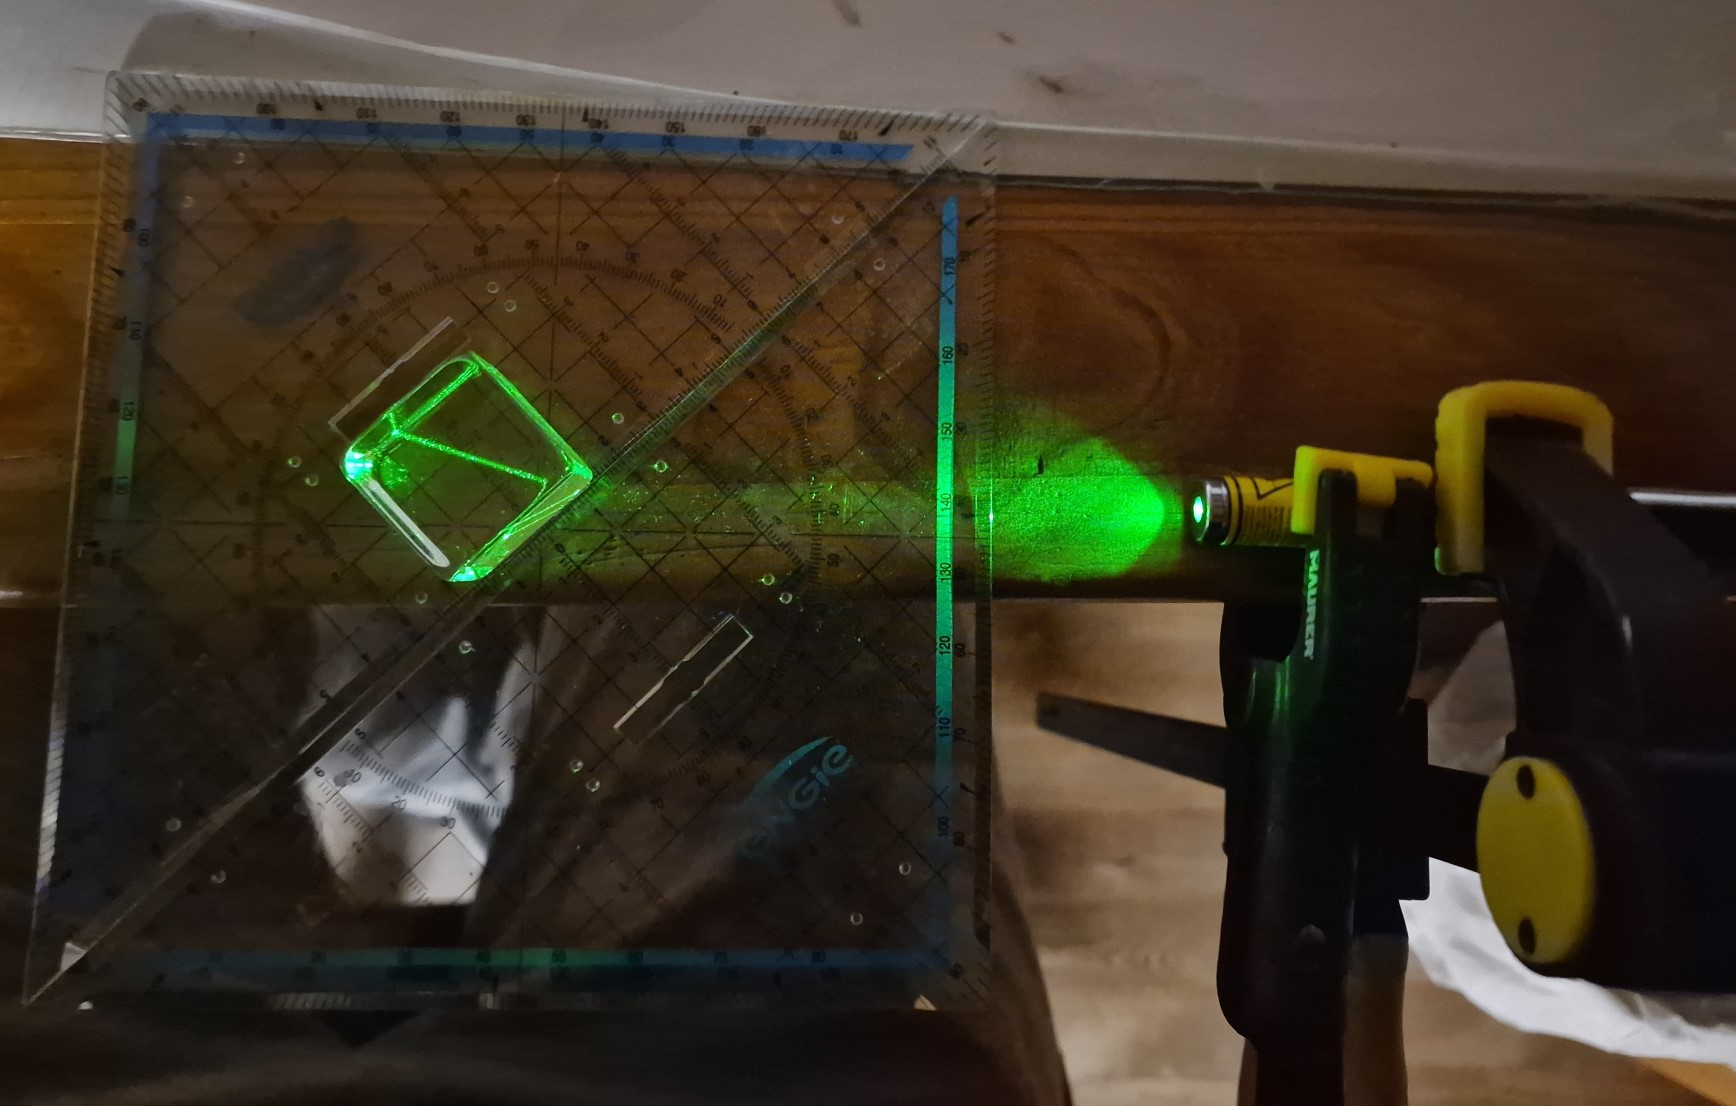
\includegraphics[height=0.7\linewidth]{imgs/winkel_messen_wurfel}
			\caption{Messung des Transmissionswinkels}
			\label{fig:winkelmessenwurfel}
		\end{subfigure}%
		\hfil
		\begin{subfigure}{0.4\textwidth}
			\centering
			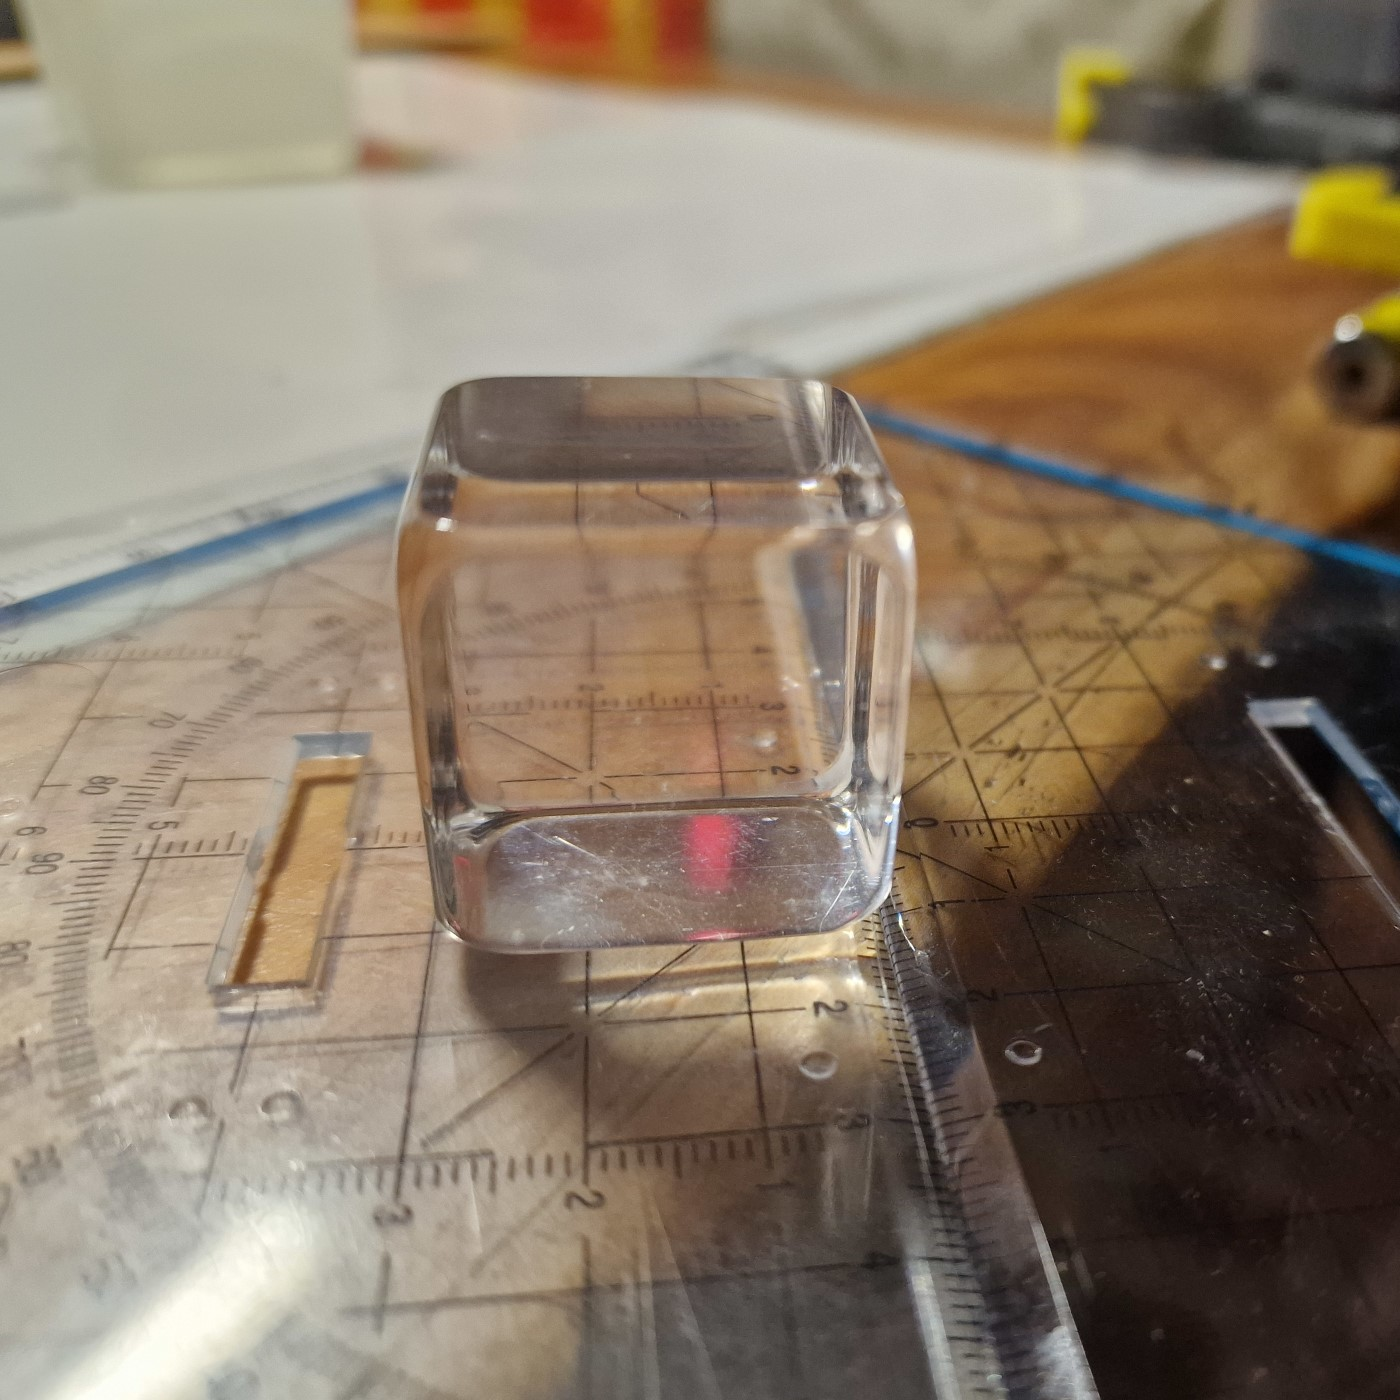
\includegraphics[height=0.7\linewidth]{imgs/wurfel_ansicht}
			\caption{Kunststoff Würfel}
			\label{fig:wurfelansicht}
		\end{subfigure}
		\caption{Messaufbau mit Kunststoffwürfel}
		\label{figs:wurfelansichten}
	\end{figure}
	
	\paragraph{Messung}
	In \cref{tab:wurfel-messergebnisse} sind die Messergebnisse zu sehen.
	\begin{table} [h]
		\centering
		\begin{tabular}{|c|c|c|c|c|c|}
			\hline
			Einfallswinkel $\Theta_{e}$ & $\si{15}{\degree}$ &
			$\si{30}{\degree}$ & $\si{45}{\degree}$ & $\si{60}{\degree}$ &
			$\si{80}{\degree}$ \\
			\hline
			Transmissionswinkel $\Theta_{t}$ & $\si{11}{\degree}$ &
			$\si{20}{\degree}$ & $\si{28}{\degree}$ & $\si{37}{\degree}$ &
			$\si{50}{\degree}$ \\
			\hline
			Brechungsindex $n$ & 1.356 & 1.462 & 1.506 & 1.439 & 1.286 \\
			\hline
			Relative Permittivität $\varepsilon_{r}$ & 1.839 & 2.137 & 2.268 & 2.071 & 1.654 \\
			\hline
		\end{tabular}
		\caption{Mess- und Rechenergebnisse für den Kunststoff Würfel}
		\label{tab:wurfel-messergebnisse}
	\end{table}
	
	Damit kommt man auf eine mittlere Relative Permittivität $\bar{\varepsilon}_{r} = 1.994$ und einen Brechungsindex $\bar{n} = 1.41$
	Dank des Brechungsindexes kann vermutet werden, dass es sich um Acrylglas handelt.
	
	
	
	\section{Weihnachtsaufgabe: Simulation}
	Hier war die Aufgabe zwei Simulationen von Antennen durchzuführen:
	
	\begin{itemize}
		\item ein Halbwellendipol im Freiraum
		\item einen Viertelwellenlängenstrahler über perfekter Groundplane
	\end{itemize}
	
	Dazu wurde die Software \texttt{EZNEC Pro/2+ v7.0} verwendet. Als individueller Parameter sollten die letzten 3 Ziffern der eigenen Matrikel Nummer genommen werden, um die Wellenlänge in \si{}{\milli\meter} zu bestimmen.
	Daraus lässt sich mit $\lambda = \si{678}{\milli\meter}$ die Betriebsfrequenz ermitteln
	\begin{equation}
		f = \frac{c_{0}}{\lambda} = \si{442.17}{\mega\hertz}
	\end{equation}
	
	\subsection{Halbwellendipol}
	In der Software muss die Datei \texttt{Dipole1.ez} geöffnet und die berechnete Frequenz eingegeben werden. Die Option \texttt{[Rescale]} muss aktiviert sein.
	
	\paragraph{Stromverteilung} Die Stromverteilung ist in \cref{fig:dipolantennaview} zu sehen. Die Verteilung entspricht einer Kosinus Halbwelle und hat das Maximum bei $y=0$ (rosa Linie)
	\begin{figure}[h]
		\centering
		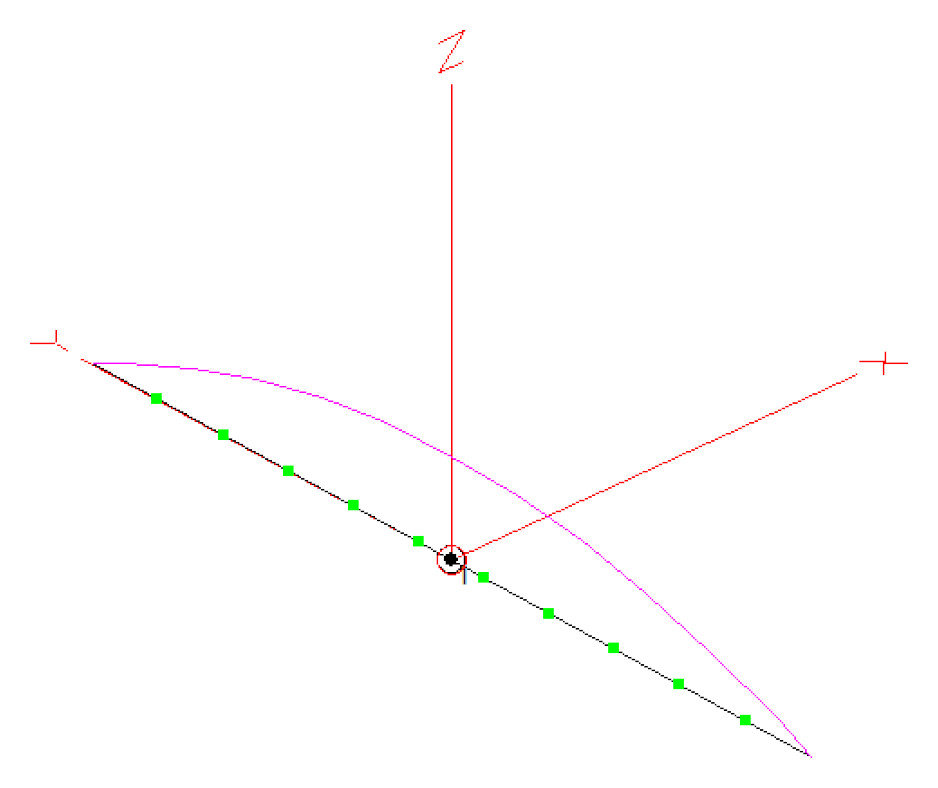
\includegraphics[width=0.7\linewidth]{imgs/dipol_antenna_view}
		\caption{Stromverteilung des Halbwellendipols}
		\label{fig:dipolantennaview}
	\end{figure}
	
	\paragraph{Polarisation}
	Um die Polarisation sehen zu können muss im Hauptfenster auf \texttt{[Desc Options] > [Plot] > [Fields]} geklickt werden, um die Option \texttt{[Vert, Horiz, Total]} auszuwählen. Damit kann aus der Richtcharakteristik in \cref{figs:richtcharakteristikdipol} die Polarisation abgelesen werden. Die Farbigen Linien geben an, bei welchen Winkeln unterschiedliche Kenngrößen auftreten (grün = Maximum, magenta = \si{3}{\decibel},...). Dadurch, dass die grüne Linie nicht $0$ ist und sich das Gesamtfeld und die horizontale Polarisation vollständig überlappen, ist das gesamte Feld horizontal polarisiert.
	
	\paragraph{Richtcharakteristik}
	In \cref{figs:richtcharakteristikdipol} ist die Richtcharakteristik zu sehen, welche der des Hertz'schen Dipols sehr ähnlich ist. Dabei stellt \cref{fig:azimutdipol} den Schnitt durch die $X/Y$-Ebene und \cref{fig:elevdipol} den Schnitt durch die $X/Z$-Ebene dar.
	\begin{figure}[h]
		\centering
		\begin{subfigure}{0.5\textwidth}
			\centering
			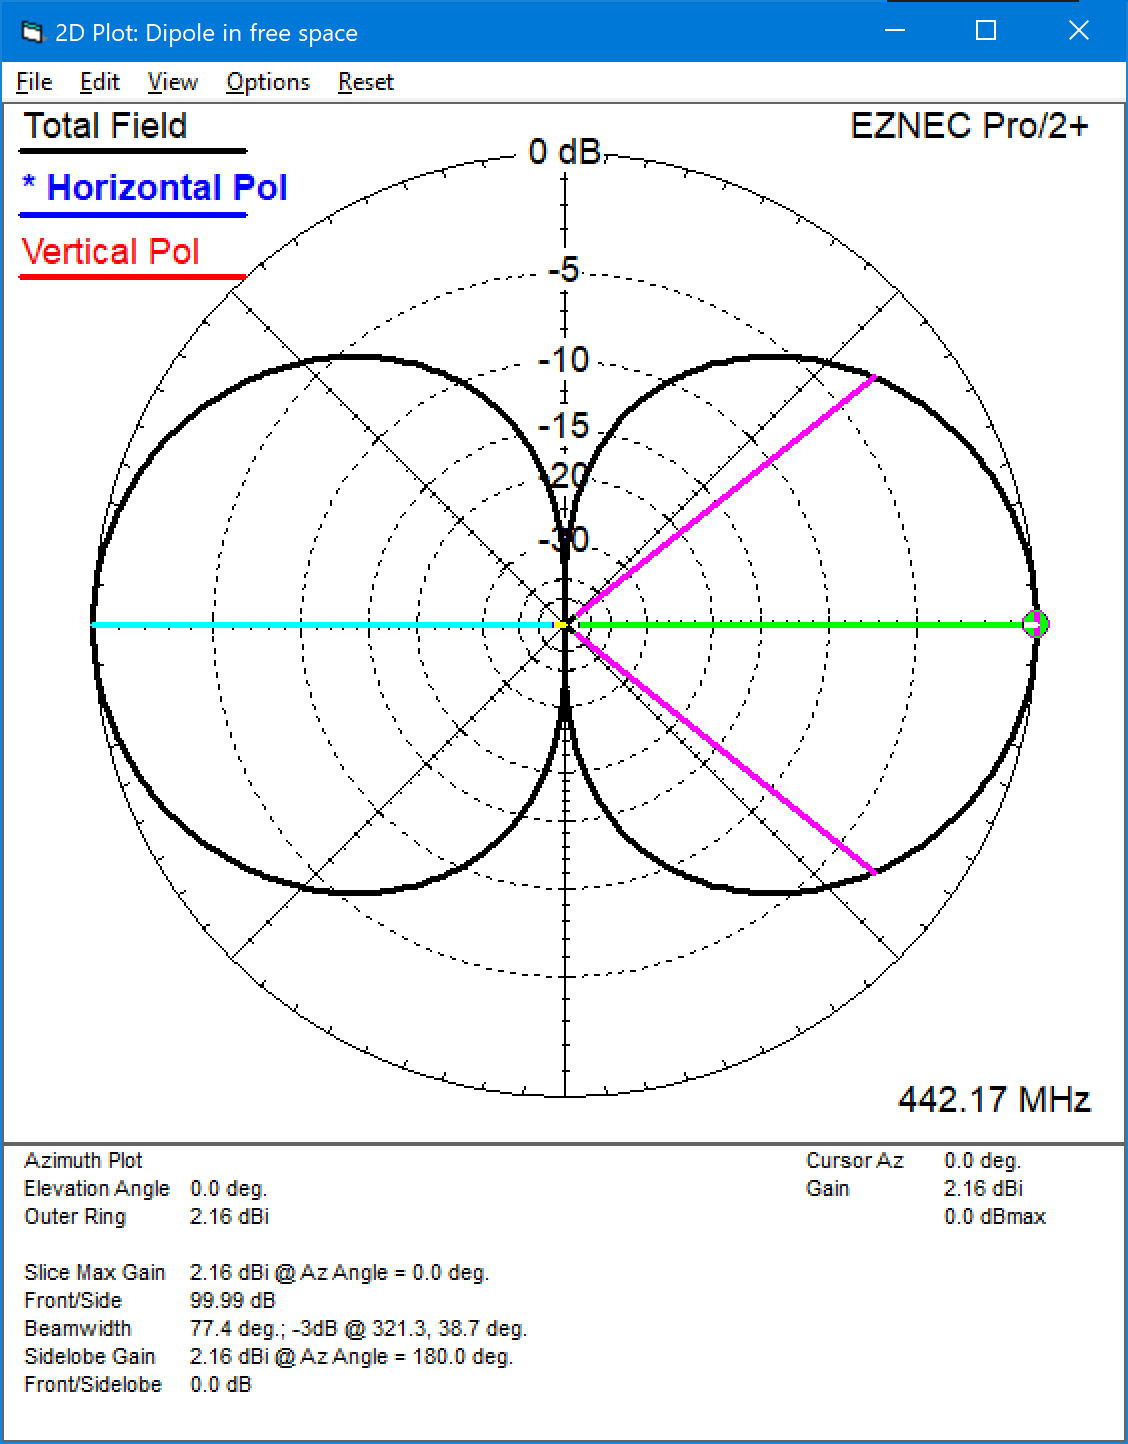
\includegraphics[height=1.2\textwidth]{imgs/azim_richtchar_dipol.png}
			\caption{$X/Y$ Schnitt}
			\label{fig:azimutdipol}
		\end{subfigure}%
		\hfil
		\begin{subfigure}{0.5\textwidth}
			\centering
			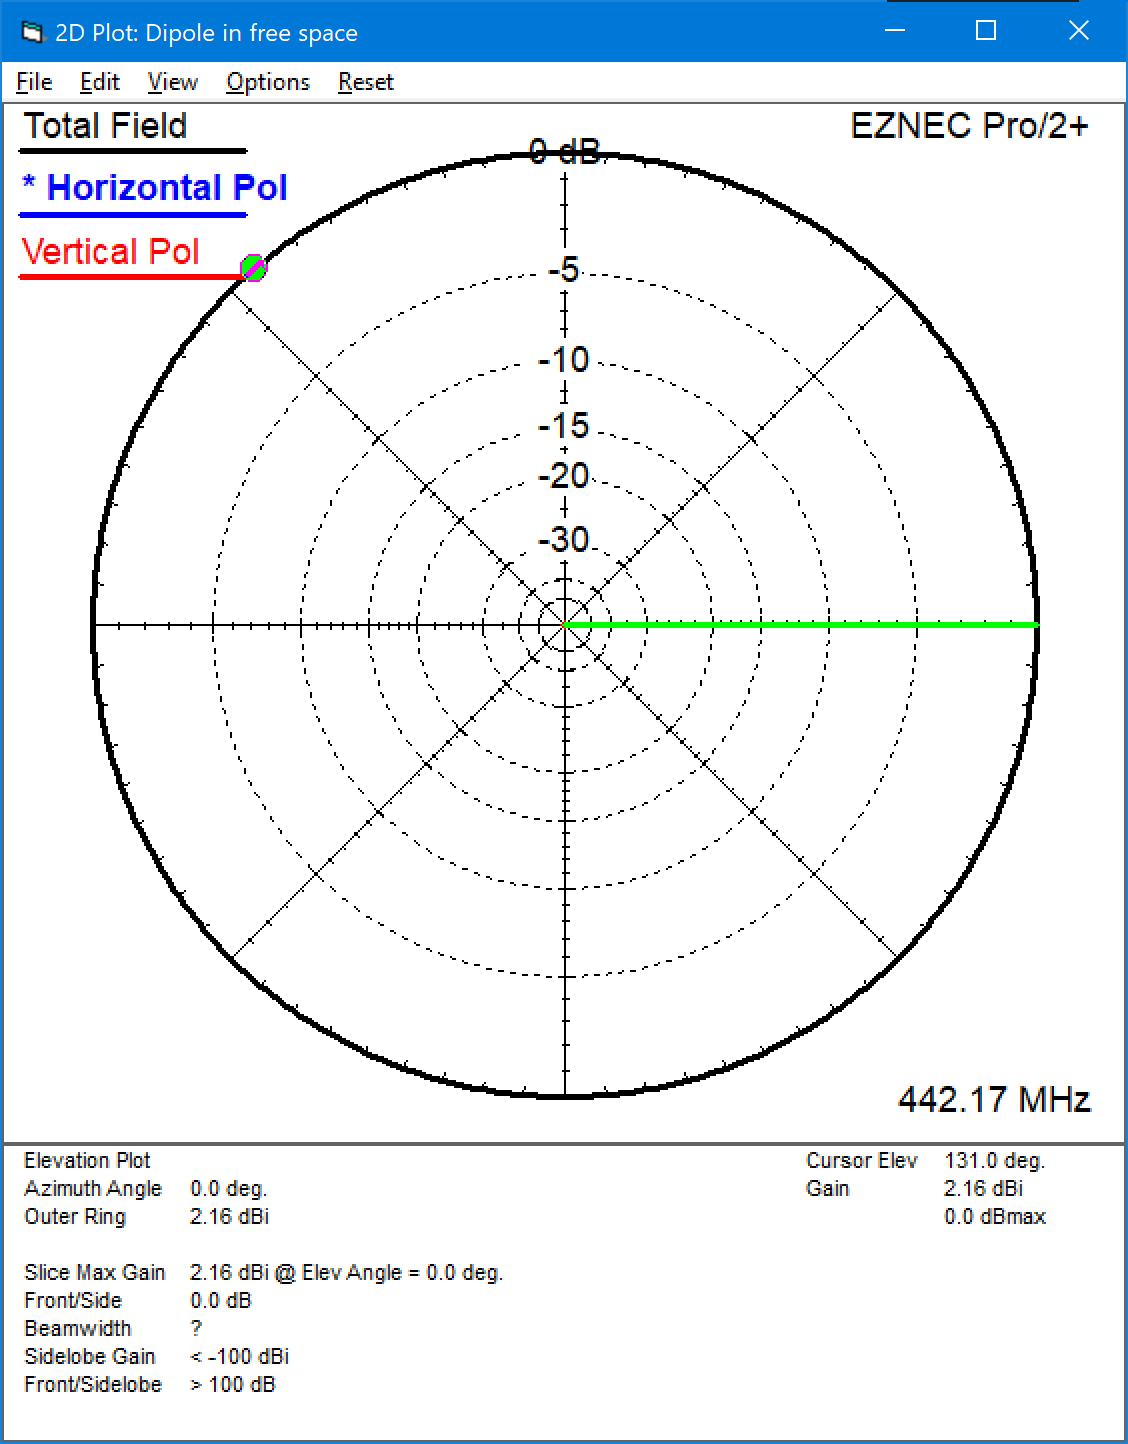
\includegraphics[height=1.2\textwidth]{imgs/elev_richtchar_dipol.png}
			\caption{$X/Z$ Schnitt}
			\label{fig:elevdipol}
		\end{subfigure}
		\caption{Richtdiagramm und Polarisation der Dipolantenne}
		\label{figs:richtcharakteristikdipol}
	\end{figure}
	
	\paragraph{Gewinn}
	Aus \cref{figs:richtcharakteristikdipol} kann der Gewinn $G$ der Antenne ermittelt werden. Dafür wird das Maximum des Gesamtfeldes abgelesen $G=\si{2.16}{\decibel i}$.
	
	\paragraph{Rayleighdistanz}
	Die Rayleighdistanz gibt an, ab welcher Entfernung von der Antenne das Fernfeld gültig ist. Diese kann mit \cref{eqn:rayleighdipol} bestimmt werden.
	
	\begin{equation} \label{eqn:rayleighdipol}
		r_{R}=\frac{2D^{2}}{\lambda}(+\lambda) = \frac{2 \left(\frac{\lambda}{2}\right)^2}{\lambda} = \frac{\lambda}{2} + \lambda = \si{1017}{\milli\meter}
	\end{equation}
	Der Term $+\lambda$ ist nötig für kleine Antennen. Diese Antenne ist $\si{339}{\milli\meter}$ lang, was genau $\frac13 r_{R}$ entspricht.
	
	\paragraph{Antennenimpedanz}
	Mit der Funktion \texttt{[Src Dat]} können die Daten der Antenne eingesehen werden. Diese sind in \cref{fig:piuzdipol} zu sehen. Die Impedanz beträgt $(81.76+\mathrm{j} 46.03)\si{}{\ohm}$.
	
	\begin{figure}[h]
		\centering
		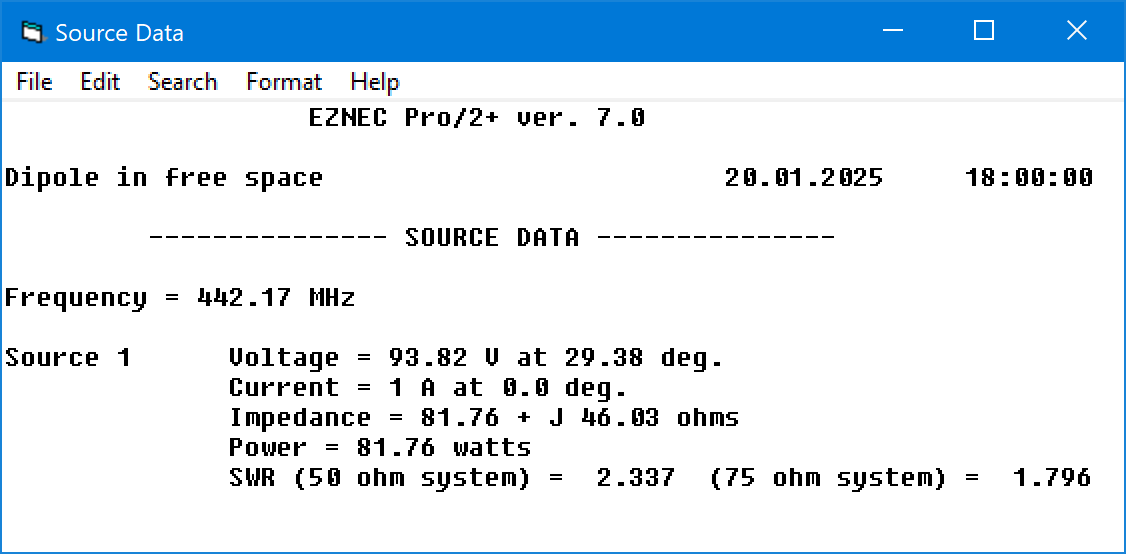
\includegraphics[width=0.7\linewidth]{imgs/PIUZ_dipol}
		\caption{Kennwerte der Dipolantenne}
		\label{fig:piuzdipol}
	\end{figure}
	
	
	%%%%%%%%%%%%%%%%%%%%%%%%%%%%%%%%%%%%
	%%%%%%%%%%%%%%%%%%%%%%%%%%%%%%%%%%%%
	
	
	\subsection{Viertelwellenlängenstrahler über perfekter Groundplane}
	In der Software muss die Datei \texttt{Vert1.ez} geöffnet und die berechnete Frequenz eingegeben werden. Die Option \texttt{[Rescale]} muss aktiviert sein.
	Weiters muss die Option \texttt{[Ground Type]} auf \texttt{[Perfect]} gestellt werden.
	
	\paragraph{Stromverteilung} Die Stromverteilung ist in \cref{fig:quartwaveantennaview} zu sehen. Die Verteilung entspricht einer Kosinus Viertelwelle und hat das Maximum bei $z=0$ (rosa Linie)
	\begin{figure}[h]
		\centering
		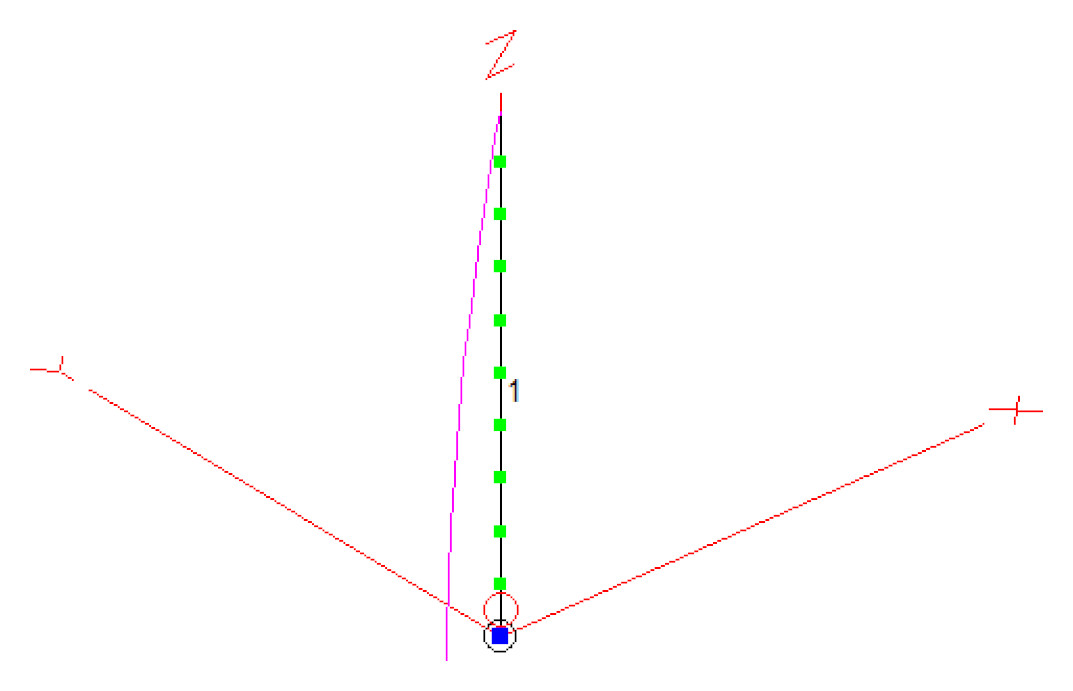
\includegraphics[width=0.7\linewidth]{imgs/quartwave_antenna_view}
		\caption{Stromverteilung der Viertelwellen Antenne}
		\label{fig:quartwaveantennaview}
	\end{figure}
	
	\paragraph{Polarisation}
	Um die Polarisation sehen zu können muss im Hauptfenster wieder auf \texttt{[Desc Options] > [Plot] > [Fields]} geklickt werden, um die Option \texttt{[Vert, Horiz, Total]} auszuwählen. Damit kann aus der Richtcharakteristik in \cref{figs:richtcharakteristikquartwave} die Polarisation abgelesen werden. Die Farbigen Linien geben an, bei welchen Winkeln unterschiedliche Kenngrößen auftreten (Grün = Maximum, Magenta = \si{3}{\decibel},...). Dadurch, dass die grüne Linie nicht $0$ ist und sich das Gesamtfeld und die vertikale Polarisation vollständig überlappen, ist das gesamte Feld vertikal polarisiert.
	
	\paragraph{Richtcharakteristik}
	In \cref{figs:richtcharakteristikquartwave} ist die Richtcharakteristik zu sehen, welche im Grunde wie die Hälfte der Dipolantenne ausschaut. Dabei stellt \cref{fig:azimutquartwave} den Schnitt durch die $X/Y$-Ebene und \cref{fig:elevquartwave} den Schnitt durch die $X/Z$-Ebene dar.
	\begin{figure}[h]
		\centering
		\begin{subfigure}{0.5\textwidth}
			\centering
			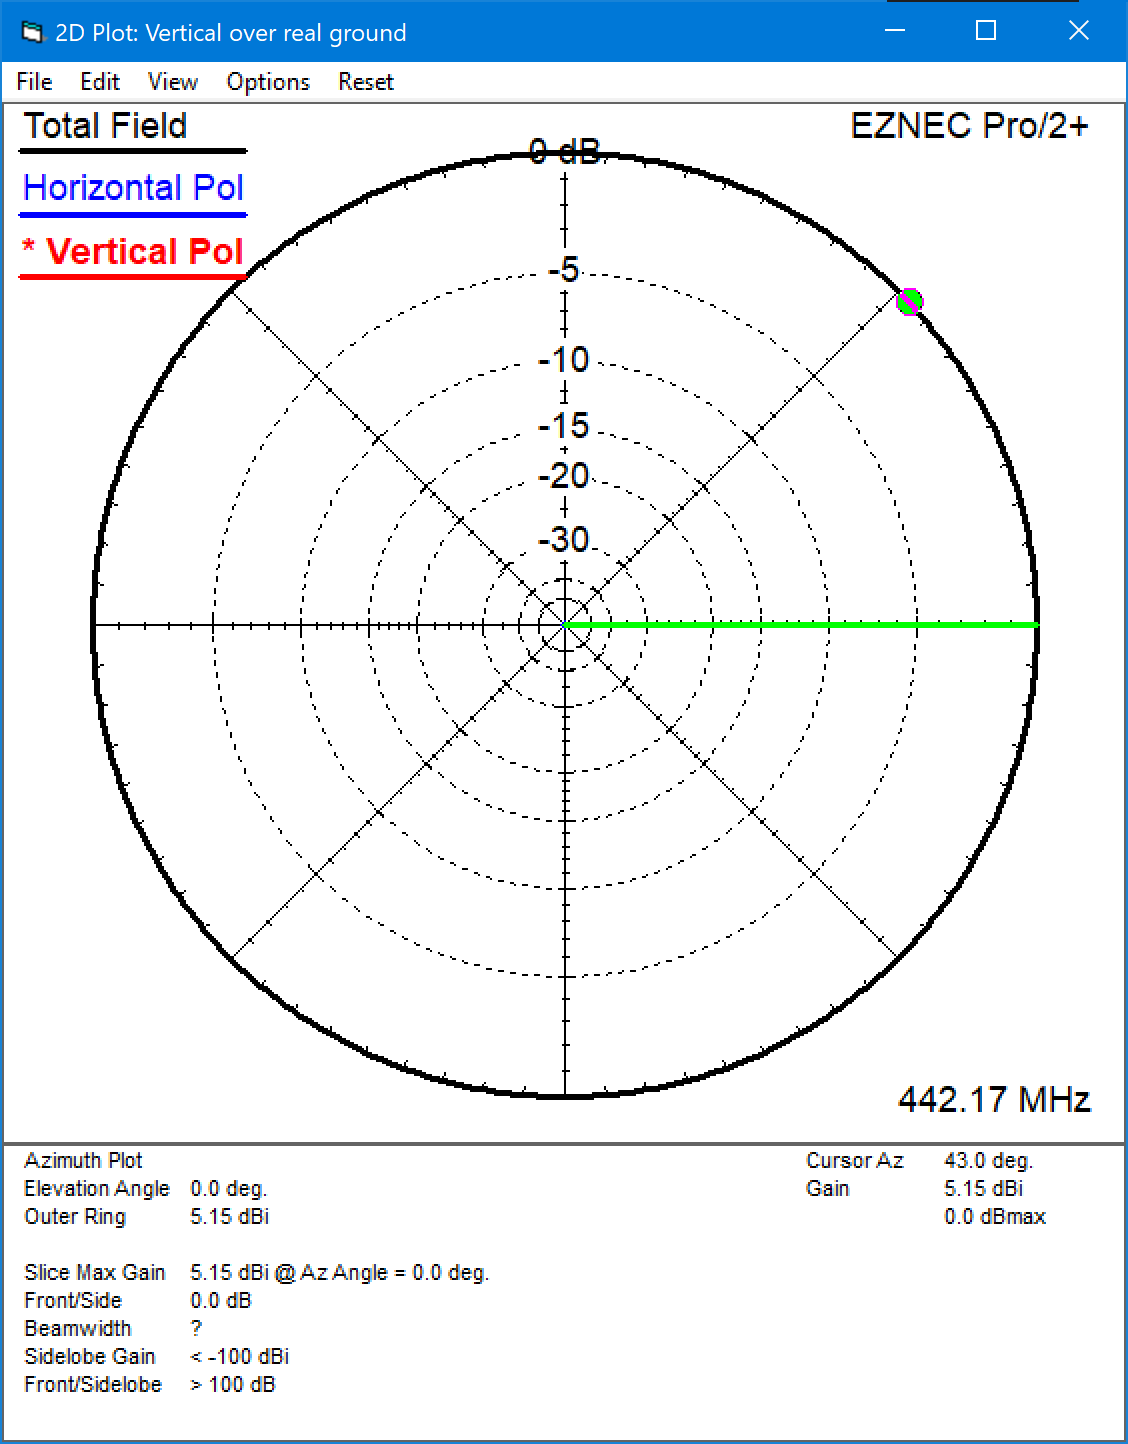
\includegraphics[height=1.2\textwidth]{imgs/azim_richtchar_quartwave.png}
			\caption{$X/Y$ Schnitt}
			\label{fig:azimutquartwave}
		\end{subfigure}%
		\hfil
		\begin{subfigure}{0.5\textwidth}
			\centering
			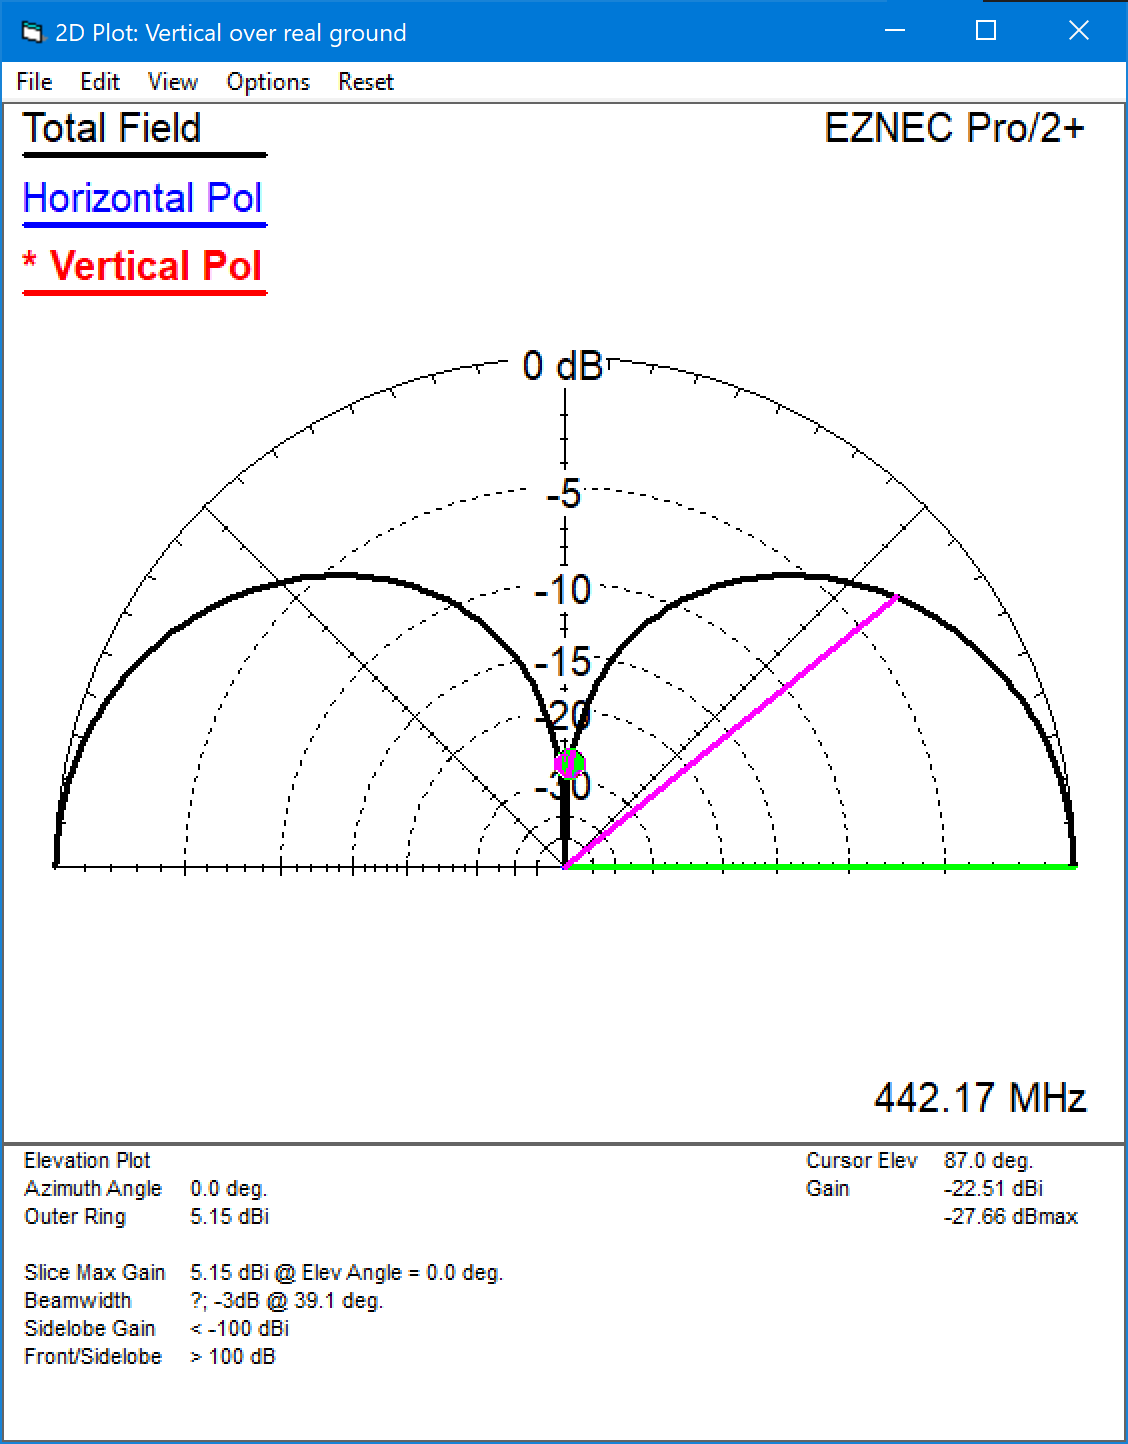
\includegraphics[height=1.2\textwidth]{imgs/elev_richtchar_quartwave.png}
			\caption{$X/Z$ Schnitt}
			\label{fig:elevquartwave}
		\end{subfigure}
		\caption{Richtdiagramm und Polarisation der Viertelwellen Antenne}
		\label{figs:richtcharakteristikquartwave}
	\end{figure}
	
	\paragraph{Gewinn}
	Aus \cref{figs:richtcharakteristikdipol} kann der Gewinn $G$ der Antenne ermittelt werden. Dafür wird das Maximum des Gesamtfeldes abgelesen $G=\si{5.15}{\decibel i}$.
	
	\paragraph{Rayleighdistanz}
	Die Rayleighdistanz kann wieder mit \cref{eqn:rayleighquartwave} bestimmt werden.
	
	\begin{equation} \label{eqn:rayleighquartwave}
		r_{R}=\frac{2D^{2}}{\lambda}(+\lambda) = \frac{2 \left(\frac{\lambda}{4}\right)^2}{\lambda} = \frac{\lambda}{8} + \lambda = \si{762.75}{\milli\meter}
	\end{equation}
	Diese Antenne ist $\si{163}{\milli\meter}$ lang.
	
	\paragraph{Antennenimpedanz}
	Mit der Funktion \texttt{[Src Dat]} werden wieder die Daten der Antenne eingesehen. Diese sind in \cref{fig:piuzquartwave} zu sehen. Die Impedanz beträgt $(36.65 + \mathrm{j} 2.973)\si{}{\ohm}$.
	
	\begin{figure}[h!]
		\centering
		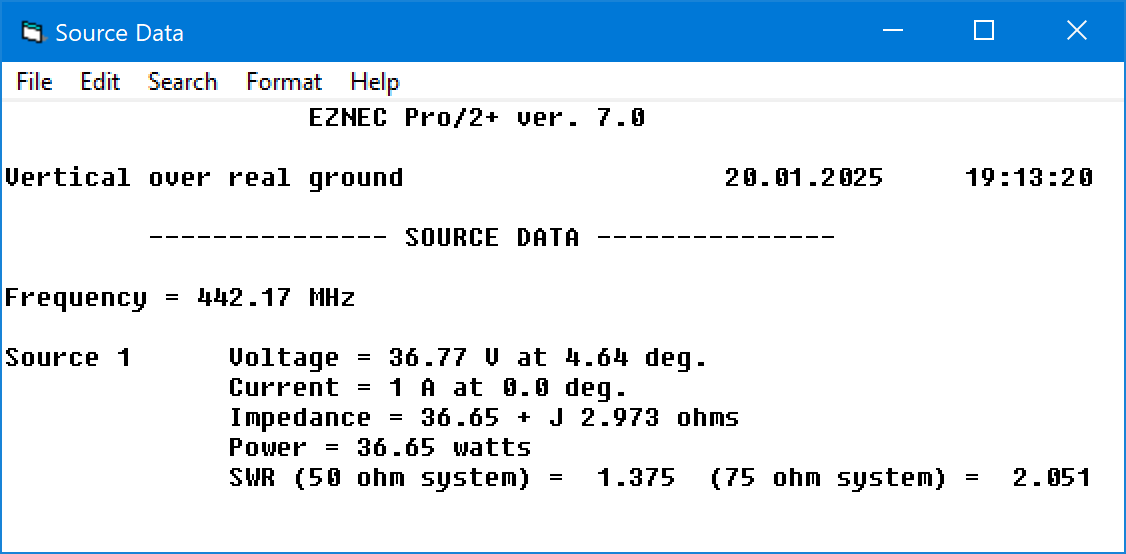
\includegraphics[width=0.7\linewidth]{imgs/PIUZ_quartwave}
		\caption{Kennwerte der Viertelwellen Antenne}
		\label{fig:piuzquartwave}
	\end{figure}
	
	
\end{document}
